%\chapter{Revis\~ao da literatura especializada - Fundamenta\c{c}\~ao te\'orica do Tema 2}
%\label{chapter:tema2}

\chapter{O Projeto \rovname}
\label{chapter:contrucaorov}

Esta seção pode conter a construção do ROV.

\section{Desenvolvimento do Projeto}
\label{sec:desenvolvimentodoprojeto}

%% ------------------------------------------------------------------------- %%
\subsection{Softwares}
\label{sec:softwares}

texto texto texto texto texto texto texto texto texto texto
texto texto texto texto texto texto texto texto texto texto
texto texto texto texto texto texto texto texto texto texto

\subsubsection{Ubuntu Linux 16.04}
\label{sec:ubuntulinux}

De acordo com \cite{whatisUbuntu}, O Ubuntu é um sistema operacional Linux completo, disponível gratuitamente (Open-Source) com suporte comunitário e profissional. O Projeto Ubuntu é patrocinado pela \cite{canonical}. A Canonical não cobrará taxas de licença pelo Ubuntu, agora ou em qualquer estágio no futuro. O modelo de negócios da Canonical é fornecer suporte técnico e serviços profissionais relacionados ao Ubuntu.

\subsubsection{ROS e Gazebo (Ambiente de Simulação)}
\label{sec:rosegazebo}

De acordo com \cite{ROSIntroduction}, O ROS é um sistema meta-operacional de código aberto. Fornece os serviços como abstração de hardware, controle de dispositivo de baixo nível, comumente usado funcionalidade, passagem de mensagens entre processos e pacote gestão.

De acordo com \cite{gazebo}, Gazebo É o simulador de física do mundo real, oferecendo a capacidade de simular com precisão e eficiência populações de robôs em ambientes internos e externos complexos sendo gratuito com uma comunidade ativa.

\subsubsection{Gephi (Pacote de software de análise e visualização de rede)}
\label{sec:gephi}

texto texto texto texto texto texto texto texto texto texto
texto texto texto texto texto texto texto texto texto texto
texto texto texto texto texto texto texto texto texto texto

\subsubsection{Draw.io (Aplicação de diagramação gráfica online)}
\label{sec:drawio}

texto texto texto texto texto texto texto texto texto texto
texto texto texto texto texto texto texto texto texto texto
texto texto texto texto texto texto texto texto texto texto

\subsubsection{Solidworks (Software CAD 3D (Design Assistido por Computador))}
\label{sec:solidwoks}

texto texto texto texto texto texto texto texto texto texto
texto texto texto texto texto texto texto texto texto texto
texto texto texto texto texto texto texto texto texto texto

\subsubsection{Cura (Software fatiador e servidor para impressora 3D)}
\label{sec:cura}

texto texto texto texto texto texto texto texto texto texto
texto texto texto texto texto texto texto texto texto texto
texto texto texto texto texto texto texto texto texto texto
%% ------------------------------------------------------------------------- %%

\subsection{Desenho Técnico}
\label{sec:desenhotecnico}

Apresentação da vista do desenho técnico do \rovname \space desenvolvido e renderizado no SolidWorks, como é mostrado nas figuras Figura~\ref{fig:Projvistatotal}, Figura~\ref{fig:Projvistafrnotal}, Figura~\ref{fig:Projvistainferior} e Figura~\ref{fig:Projvistasuperior}, vista geral, vista frontal, vista inferior e superior respectivamente.

\begin{figure}[!htb]
	\centering	
	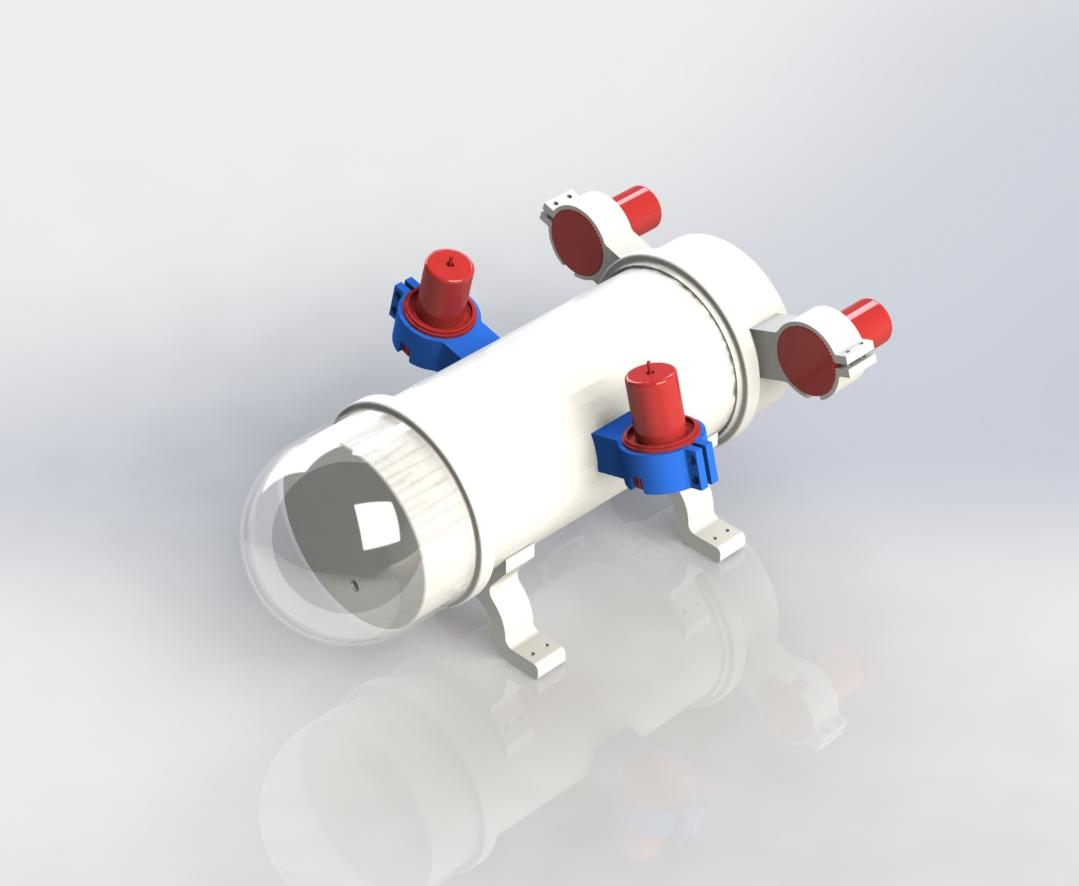
\includegraphics[width=0.5\textwidth]{Figures/Rov/Proj_vista_total.jpeg}
	\caption{Vista Total, Fonte: Elaborada pelo autor\the\year}
	\label{fig:Projvistatotal}
\end{figure}

\begin{figure}[!htb]
	\centering	
	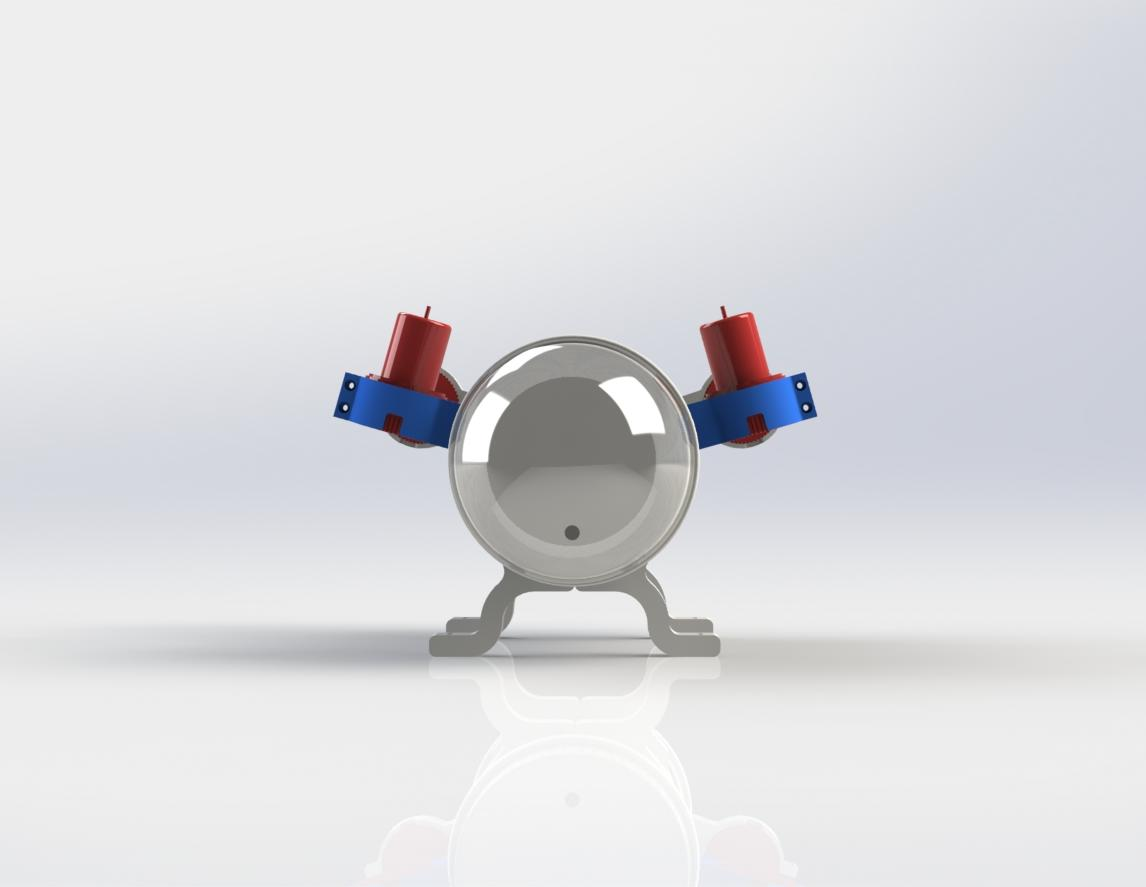
\includegraphics[width=0.5\textwidth]{Figures/Rov/Proj_vista_frontal.jpeg}
	\caption{Vista Frontal, Fonte: Elaborada pelo autor\the\year}
	\label{fig:Projvistafrnotal}
\end{figure}

\begin{figure}[!htb]
	\centering	
	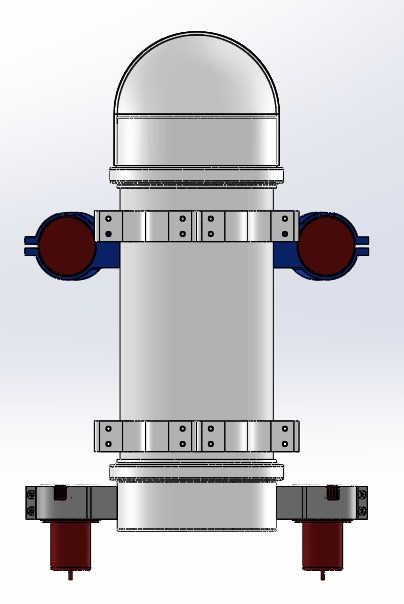
\includegraphics[angle=90,width=0.5\textwidth]{Figures/Rov/Proj_vista_inferior.jpeg}
	\caption{Vista Inferior, Fonte: Elaborada pelo autor\the\year}
	\label{fig:Projvistainferior}
\end{figure}

\begin{figure}[!htb]
	\centering	
	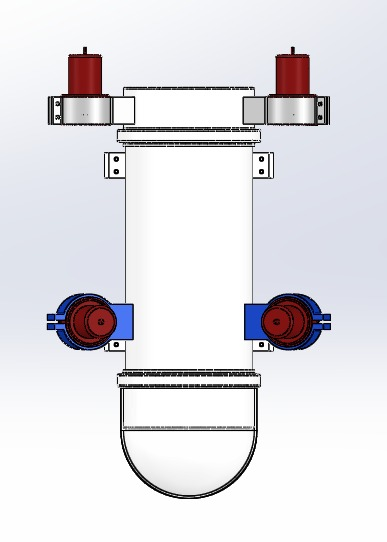
\includegraphics[angle=90,width=0.5\textwidth]{Figures/Rov/Proj_vista_superior.jpeg}
	\caption{Vista Superior, Fonte: Elaborada pelo autor\the\year}
	\label{fig:Projvistasuperior}
\end{figure}

%% ------------------------------------------------------------------------- %%

\subsection{Estrutura (Chassi)}
\label{sec:estruturachassi}

texto texto texto texto texto texto texto
texto texto texto texto texto texto texto
texto texto texto texto texto texto texto

Materiais utilizados para a construção.

\begin{itemize}
    \item 1 - Tubo PVC 150mm;
    \item 4 - Bomba De Porão Seaflo 1100gph - 4164lph 12v;
    \item 2 - Tampas PVC 150mm com borracha;
    \item 4 - Suportes impressos em PLA 3d;
    \item 4 - Hélices de plástico;
    \item 1 - Arduíno Mega 2560;
    \item 2 - Ponte H Monster Motor Shield VNH2SP30 30a 2 Motor;
    \item 1 - Cúpula Acrílica Hemisférica;
    \item 40 - Parafusos de aço inox com porca;
    \item 15 - Metros de fios awg22;
\end{itemize}

\begin{figure}[!htb]
	\centering	
	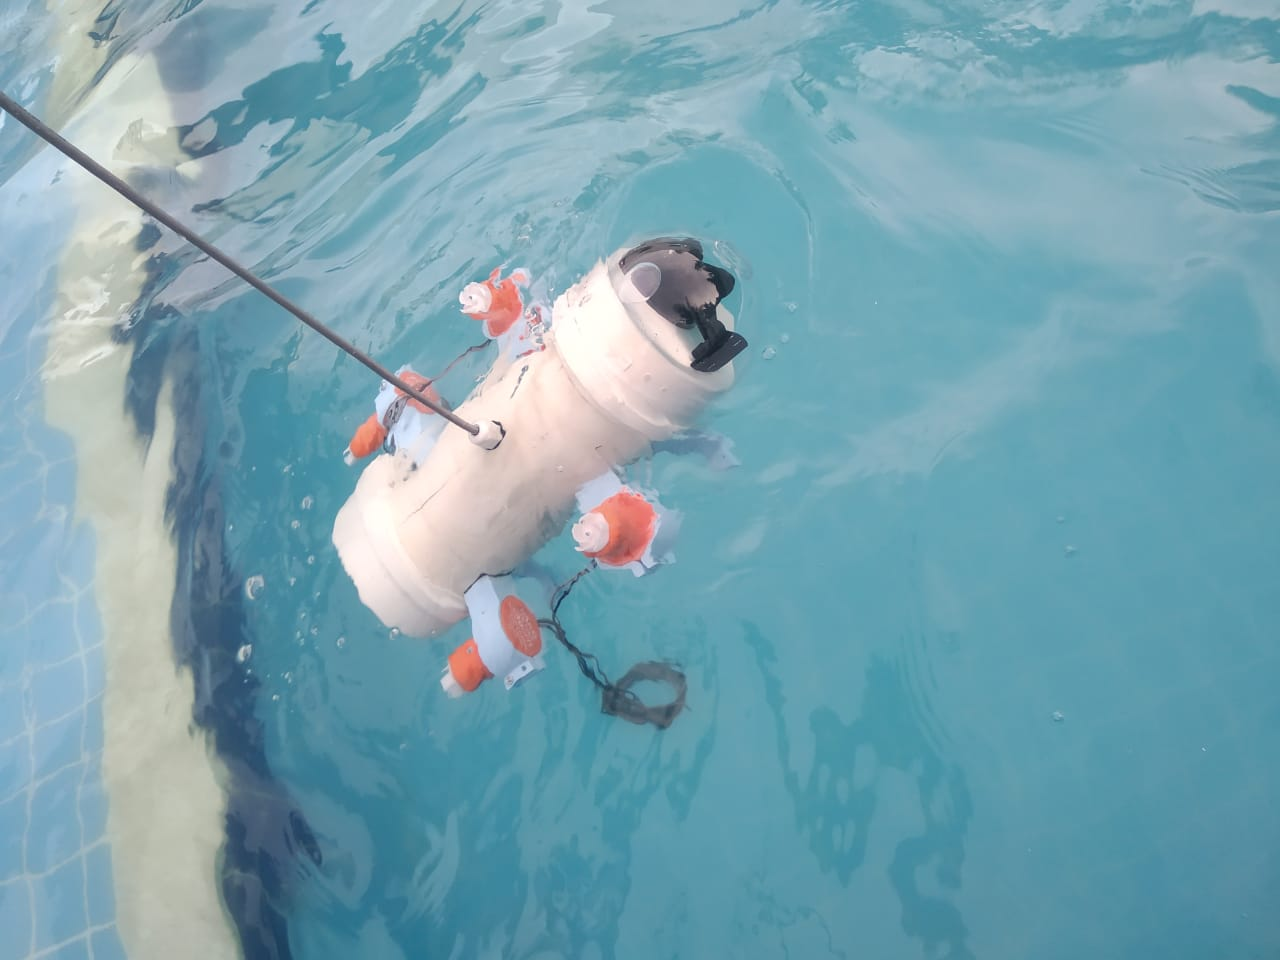
\includegraphics[width=0.5\textwidth]{Figures/Rov/Estrutura_ROV.jpeg}
	\caption{Vista Superior, Fonte: Elaborada pelo autor\the\year}
	\label{fig:estruturarov}
\end{figure}
%% ------------------------------------------------------------------------- %%

\subsection{Motores de Tração}
\label{sec:motoresdetracao}

De acordo com \cite{bombadeporao}, As bombas de esgoto não-automáticas 1100GPH da SEAFLO oferecem evacuação de água ativada por um painel ou interruptor de bóia alem de Incluir proteção de bloqueio anti-ar e vedações herméticas exclusivas, fiação de bloco de grau marítimo. Disponível para tensão 12 e 24 tensão. O modelo 1100GPH 12V, atende as especificações do projeto devido ao seu alto torque e selagem hermética, possibilitando uma submersão de até 20 pés (6,096) metros.

Principais Características:

\begin{itemize}
    \item 2 anos de garantia
    \item Atende ou excede os padrões RoHS, SGS e ISO
    \item Operação tradicional por interruptor ou interruptor de bóia
    \item Totalmente submersível
    \item Base do filtro de encaixe para fácil manutenção
    \item Bomba e interruptor são produtos independentes
    \item Motores eficientes e de longa vida útil selados
    \item Funciona a seco, capaz de cargas de trabalho normais
    \item Operação silenciosa
    \item limites de temperatura de $110\,^{\circ}\mathrm{F}$ ($43\,^{\circ}\mathrm{C}$)
    \item eixo de aço inoxidável
    \item Proteção anti-Airlock
    \item Selos herméticos exclusivos
    \item Fiação bloqueada de grau marítimo
\end{itemize}

\begin{figure}[!htb]
	\centering
	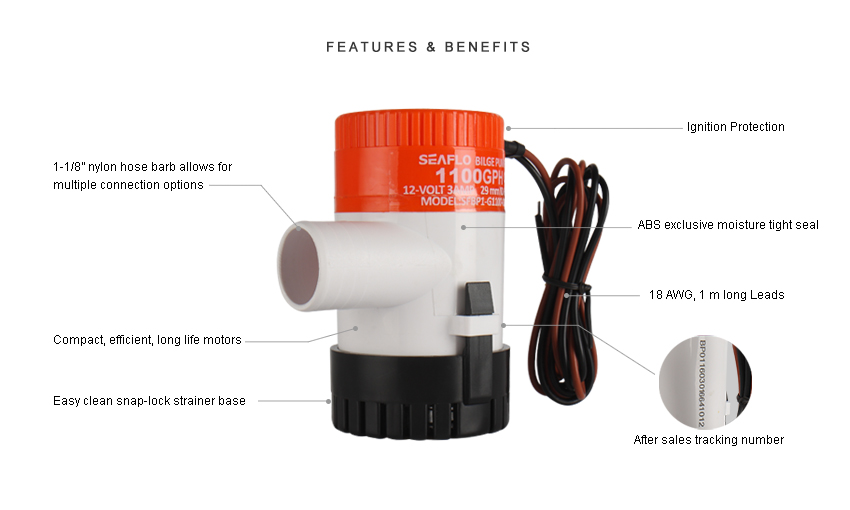
\includegraphics[width=0.8\textwidth]{Figures/Rov/Bomba_porao-Seaflo.jpg}
	\caption{Vista Superior, \cite{bombadeporao}}
	\label{fig:bombaporao}
\end{figure}
%% ------------------------------------------------------------------------- %%

\subsection{Cabos e Conexões}
\label{sec:caboseconexoes}

%% ------------------------------------------------------------------------- %%

\subsection{Sensores}
\label{sec:sensores}
%% ------------------------------------------------------------------------- %%

\subsection{Microcontroladores}
\label{sec:microcontroladores}

O sistema embarcado utilizado para controlar as entradas e saídas de comandos lógicos do \rovname.

\subsubsection{Arduino}
\label{sec:arduino}
(+ texto)

\subsubsection{Raspberry Pi}
\label{sec:raspberrypi}
(+ texto)
%% ------------------------------------------------------------------------- %%

\subsection{Ponte-H}
\label{sec:ponteh}

De acordo com \cite{monstermotorshield}, O VNH2SP30 é um driver de motor de ponte que incorpora um driver monolítico duplo alto e dois interruptores laterais baixos, os pinos do sensor de corrente (CS) produzirão aproximadamente 0,13 volts por amp de corrente de saída. Sendo uma ótima escolha já que o mesmo é capaz de controlar até dois motores com corrente de pico de 30A, controlando o sentido de rotação e velocidade do motor.

Principais Características:

\begin{itemize}
	\item Tensão máxima: 30V;
    \item Máxima corrente: 30 A;
    \item Corrente nominal de operação: 14 A;
    \item Medição de corrente disponível para o Arduino nos pinos analógicos;
    \item MOSFET sobre resistência: 19 m$\Omega$;
    \item Frequência PWM máxima: 20 kHz;
    \item Proteção térmica;
    \item Proteção contra sobretensão e subtensão;
\end{itemize}

\begin{figure}[!htb]
	\centering	
	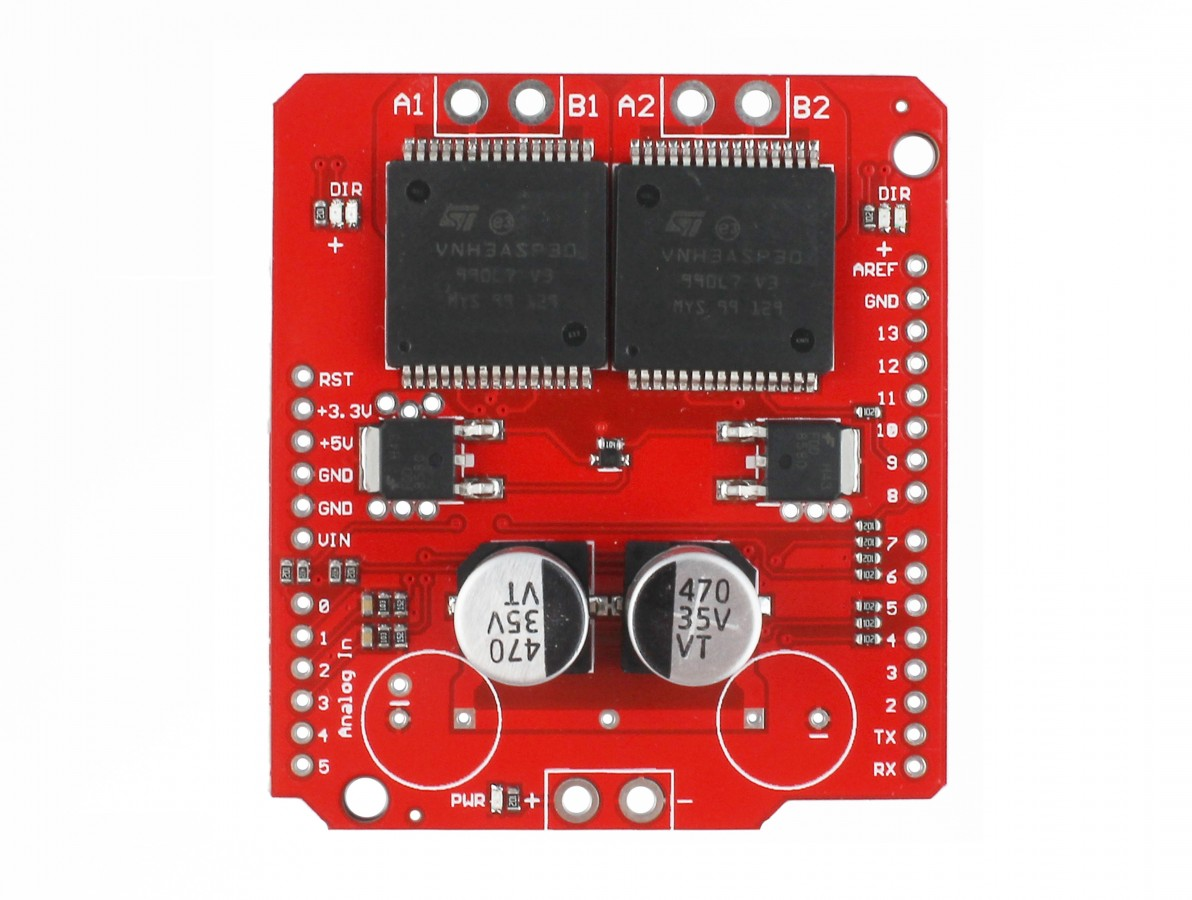
\includegraphics[width=0.5\textwidth]{Figures/Rov/Monster_motor_shield.jpg}
	\caption{Vista Superior Monster Motor Shield \cite{monstermotorshield}}
	\label{fig:monstermotorshield}
\end{figure}
%% ------------------------------------------------------------------------- %%

\subsection{Fonte de Alimentação}
\label{sec:fontedealimentacao}
%% ------------------------------------------------------------------------- %%

\subsection{Painel de Controle}
\label{sec:paineldecontrole}
%% ------------------------------------------------------------------------- %%
